 \documentclass[11pt]{article}
 \usepackage{amsmath, alltt, amssymb, xspace, times, epsfig,
   algpseudocode, color, multirow, listings, mathtools}

\usepackage[font=small,labelfont=bf,textfont=it]{caption}
\usepackage{subcaption}
\DeclarePairedDelimiter{\ceil}{\lceil}{\rceil}
\DeclarePairedDelimiter{\floor}{\lfloor}{\rfloor}

 \setlength{\evensidemargin}{0in} \setlength{\oddsidemargin}{0in}
 \setlength{\textwidth}{6.5in} \setlength{\textheight}{8.5in}
 \setlength{\topmargin}{0in} \setlength{\headheight}{0in}


\begin{document}
 \thispagestyle{empty}

 \noindent \textbf{CS525: Parallel Computing\hspace*{\fill}Spring 2013} 
 \begin{center}
   {\LARGE Homework \#5\\\small Josh Reese}\\
 \end{center}
 \begin{figure}[h]
   \centering
   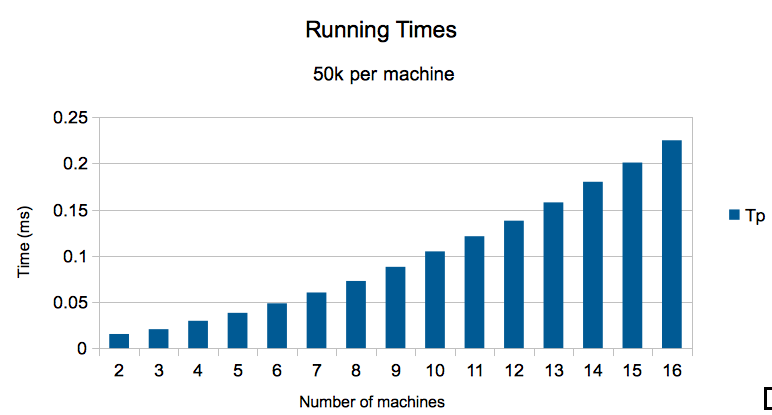
\includegraphics[width=\textwidth]{graph.png}
   \caption{Chart of run times by number of processors on a fixed
     table size.}
 \end{figure}
\end{document}
